W raporcie opisujemy jedynie te tabele, które zostały utworzone bezpośrednio przez nas, ponieważ baza danych zawiera dodatkowo tabele, które tworzone są przez Django w momencie inicjalizacji projektu.
Poniżej zamieszczony został diagram przedstawiający tabele i relacje między nimi:
\begin{figure}[H]
\centering
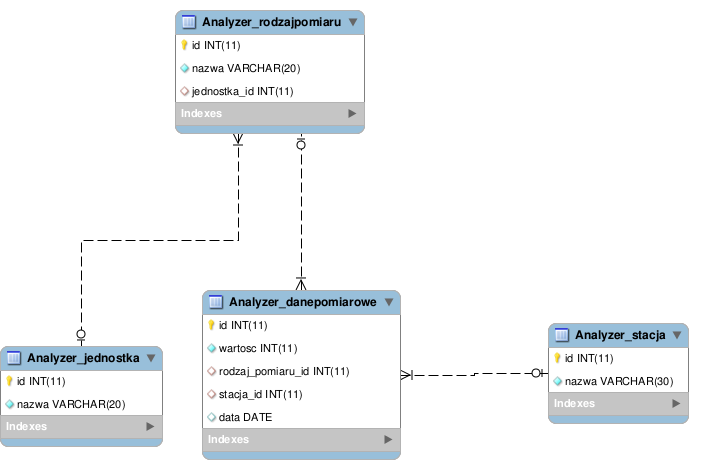
\includegraphics[width=\linewidth]{diagramEER}
\caption{Diagram tabel}
\label{fig:diagramTabel}
\end{figure}

 Poniższa tabela zawiera pełne zestawienie pól stworzonych tabel.
\begin{longtable}{|p{0.25\linewidth}|p{0.25\linewidth}||p{0.5\linewidth}|}
\hline
\textbf{Nazwa tabeli} & \textbf{Nazwa pola} & \textbf{Opis pola} \tabularnewline \hline \hline
\multirow{5}{*}{Analyzer\_danepomiarowe} & id & klucz główny (automatycznie inkrementowany) \tabularnewline\cline{2-3}
 & wartosc & całkowita część danej pomiarowej \tabularnewline\cline{2-3}
 & rodzaj\_pomiaru\_id & klucz obcy (tabela Analyzer\_rodzajpomiaru) \tabularnewline\cline{2-3}
 & stacja\_id & klucz obcy (tabela Analyzer\_stacja)\tabularnewline\cline{2-3}
 & data & data (godzina jest ignorowana) \tabularnewline\hline
\multirow{2}{*}{Analyzer\_jednostka} 
 & id & klucz główny (automatycznie inkrementowany) \tabularnewline\cline{2-3}
 & nazwa & jednostka pomiaru (np. C lub F dla temperatury) \tabularnewline\hline
\multirow{3}{*}{Analyzer\_rodzajpomiaru}
 & id & klucz główny (automatycznie inkrementowany) \tabularnewline\cline{2-3}
 & nazwa & nazwa rodzaju pomiaru, która będzie wykorzystywana do wyboru danych pomiarowych w aplikacji internetowej \tabularnewline\cline{2-3}
 & jednostka\_id & klucz obcy (tabela Analyzer\_jednostka \tabularnewline\hline
\multirow{2}{*}{Analyzer\_stacja}
 & id & klucz główny (automatycznie inkrementowany) \tabularnewline\cline{2-3}
 & nazwa & nazwa stacji, która będzie wykorzystywana do wyboru danych pomiarowych w aplikacji internetowej \tabularnewline\hline
\end{longtable}

\subsection{Opis tabel}
Tabele zostały specjalnie podzielone w taki sposób, aby móc w przyszłości łatwo dodawać kolejne wpisy. Poniżej krótko opisujemy stworzone tabele:
\begin{itemize}
	\item \textbf{Analyzer\_danepomiarowe} - w tabeli tej znajduje się pełne zestawienie danych pomiarowych. Dzięki wykorzystaniu kluczów obcych \textit{ rodzaj\_pomiaru\_id} oraz \textit{stacja\_id} można potem z tabeli filtrować potrzebne dane. Ponieważ w projekcie skupiliśmy się na pomiarach temperatury pole \textit{wartosc} reprezentowane jest przez liczbę całkowitą INT ze znakiem. Kolumna \textit{data} musi zawierać datę wykonania pomiaru, może również być w niej zapisana godzina, aczkolwiek zostanie ona w naszym programie zignorowana. W tej sytuacji można zauważyć, że domyślnie w naszej tabeli znajdują się daty w stylu \verb 2013-12-01  \verb 00:00:00  - godzina wynosi 0. Założyliśmy, że nie będą potrzebne nam pomiary z rozdzielczością godzinową.
	\item \textbf{Analyzer\_jednostka} - jednostka pomiaru została specjalnie wydzielona do osobnej tabeli, ponieważ w bazie może zdarzyć się sytuacja gdy przykładowo stworzony zostanie rodzaj pomiaru TMIN (temperatura minimalna) oraz TMAX (temperatura maksymalna), które mimo, że są różnymi rodzajami pomiaru, posiadają taką samą jednostkę - stopnie Celsjusza. Jednostka może zostać zapisana w maksymalnie 20 znakach, co oczywiście w takim wypadku jest bardzo dużym zapasem. Ponieważ jednostek w przypadku pogody nie będzie dużo nie należy przejmować się, że taka długość napisu może zająć zbyt dużo pamięci w bazie. 
	\item \textbf{Analyzer\_rodzajpomiaru} - rodzajami pomiaru mogą być np. temperatura, ciśnienie, szybkość wiatru itd. Nazwa, która zostanie wpisana w kolumnie \textit{nazwa} będzie widoczna później w aplikacji web. Z tego powodu można wpisać w jej ramach do 20 znaków. Rodzaj pomiaru powiązany jest kluczem obcym z jednostką. Później jest wykorzystywany przy wczytywaniu danych z pliku CSV.
	\item \textbf{Analyzer\_stacja} - tabela przechowuje poza kluczem głównym jedynie nazwy poszczególnych stacji. Na nazwę przyjęliśmy typ VARCHAR(30), czyli może składać się maksymalnie z 30 znaków. Nazwa stacji jest widoczna w aplikacji webowej oraz jest istotna przy wczytywaniu danych z pliku CSV.
\end{itemize}

